\section{TITLE}

%%%%%%%%%%%%%%%%%%%%%%%%%%%%%%%%%%%%%%%%%%%%%%%%%%%%%%%%%%
%%%%%%%%%%%%%%%%%%%%outline%%%%%%%%%%%%%%%%%%%%%%
%%%%%%%%%%%%%%%%%%%%%%%%%%%%%%%%%%%%%%%%%%%%%%%%%%%%%%%%%%
\begin{frame}\frametitle{Outline of lecture xx}
  \begin{itemize}
   \item EXAMPLE1
    \begin{itemize}
    \item[-] EXAMPLE1.1
    \item[-] EXAMPLE2.1
    \end{itemize}
  \end{itemize}
  \begin{itemize}  
   \item EXAMPLE2
    \begin{itemize}
    \item[-] EXAMPLE2.1
    \item[-] EXAMPLE2.2
    \end{itemize}
  \end{itemize}
\end{frame}

\subsection{EXAMPLE1}

\begin{frame}\frametitle{Sample frame, both captions}
  \begin{figure}[h!]
    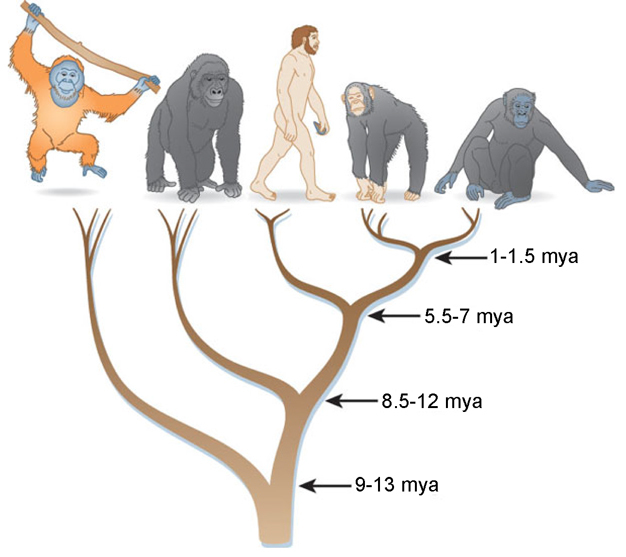
\includegraphics[height=5cm]{figures/TS-Apes.jpg}
	\figureCaption{\cite{Paabo2003}}{This is a tree. We can tell it's a tree because it has some branches. And we'll have a very long label to match it.}
  \end{figure}
\end{frame}

\begin{frame}\frametitle{Sample frame, no first caption}
  \begin{figure}[h!]
    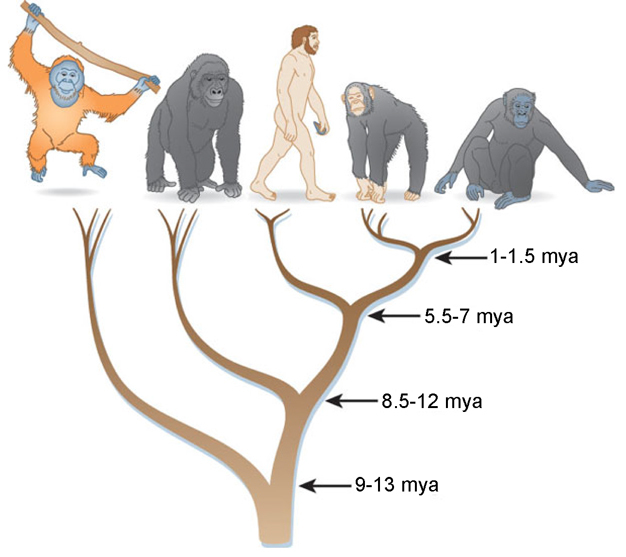
\includegraphics[height=5cm]{figures/TS-Apes.jpg}
    \def\figurename{}
	\figureCaption{}{This is a tree. We can tell it's a tree because it has some branches. And we'll have a very long label to match it.}
  \end{figure}
  We skipped the first, reference caption here.
\end{frame}

\begin{frame}\frametitle{Sample frame, no second caption}
  \begin{figure}[h!]
    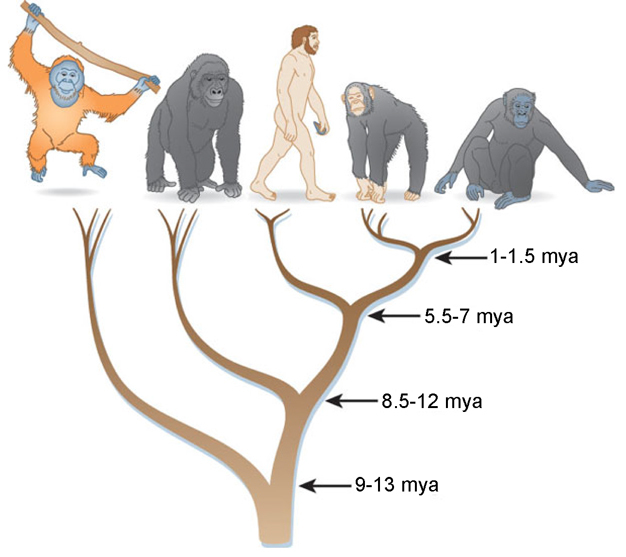
\includegraphics[height=5cm]{figures/TS-Apes.jpg}
	\figureCaption{\cite{Paabo2003}}{}
  \end{figure}
  We skipped the second caption here.
\end{frame}

\begin{frame}\frametitle{Sample frame, side-by-side list and figure}
  \begin{columns}[t]
  \column{0.65\linewidth}
    \begin{itemize}
      \item DNA (Deoxyribonucleic acid) first isolated by Friedrich Miescher\\ (born in Basel in 1844; Institute here in Basel named after him)
      \item DNA is a double helix\\ (published by Watson \& Crick in 1953 in Nature; based on images by Rosalind Franklin; Nobel price in 1962)
    \end{itemize}
  \column{0.35\linewidth}
    \begin{figure}[h!]
      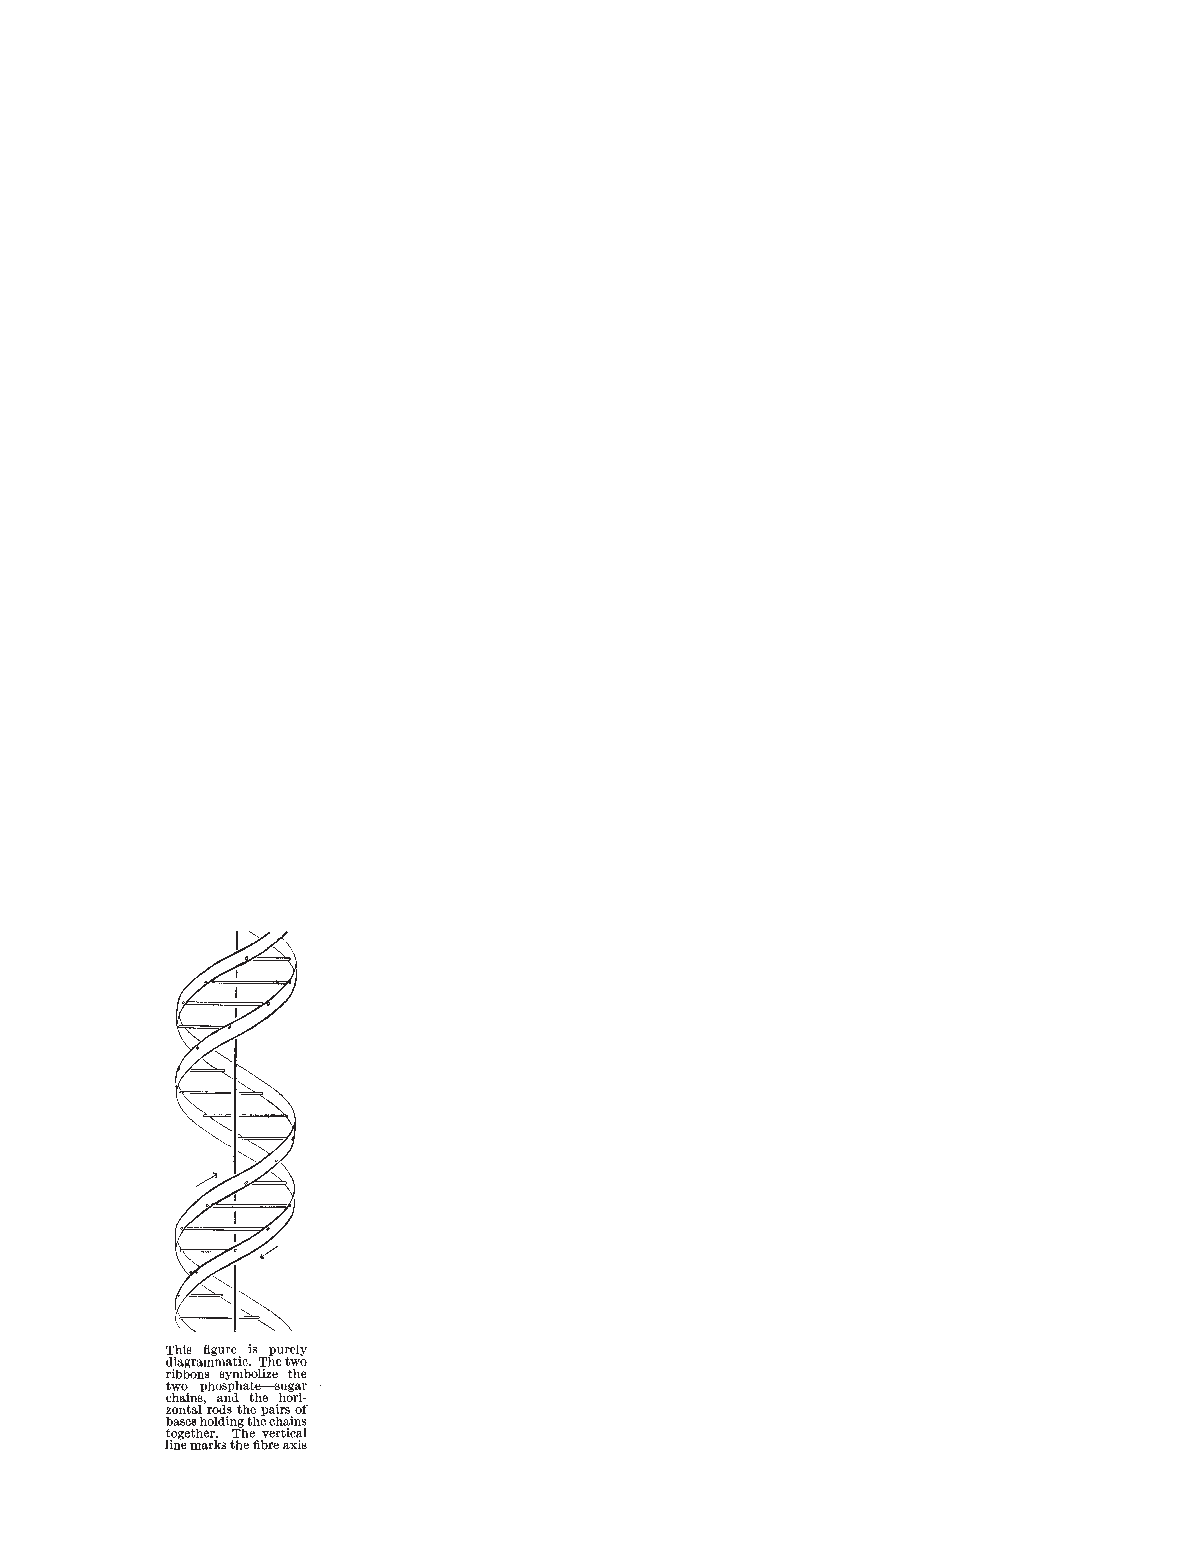
\includegraphics[width=0.5\textwidth]{figures/TS-DNA1953.pdf}
      \figureCaption{\cite{Watson1953}}{This is a DNA helix, imagine that.}
    \end{figure}
  \end{columns} 
\end{frame}

\begin{frame}\frametitle{Sample frame, a fixme and a comment}
    \fixme{Oh no, some stuff needs fixing!}
    
    \comment{J\=ulija}{This requires attention!}
\end{frame}